\section{Applying HDM on Testnet}
\nblink{brats/22a\_testnet\_hdm\_circles\_fixed.ipynb}

This chapter shows the Hausdorff distance mask method applied on three examples of the testnet.

\subsection{Results}
\begin{figure}[H]
    \centering
    \begin{subfigure}[t]{.28\textwidth}
        \centering
        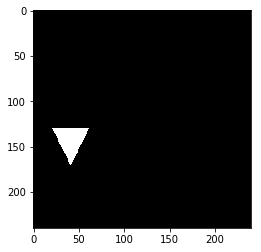
\includegraphics[width=\linewidth]{chapters/06_hdm/testnet/0.png}
        \caption{Ground truth segment}
    \end{subfigure}\hfill%
    \begin{subfigure}[t]{.34\textwidth}
        \centering
        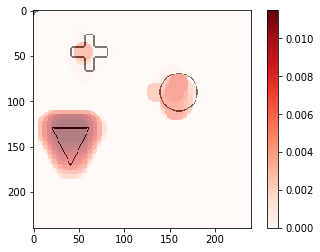
\includegraphics[width=\linewidth]{chapters/06_hdm/testnet/2.png}
        \caption{Regions where the applied masks reduce the accuracy of the segmentation}
    \end{subfigure}\hfill%
    \begin{subfigure}[t]{.36\textwidth}
        \centering
        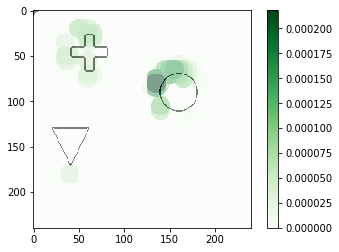
\includegraphics[width=\linewidth]{chapters/06_hdm/testnet/3.png}
        \caption{Regions where the applied masks increase the accuracy of the segmentation}
    \end{subfigure}
    \caption{Both the visualizations (b) and (c) show that both the segmentation region itself and the circle are important for the correct segmentation.}
    \label{testnet_
\end{figure}

\begin{figure}[H]
    \centering
    \begin{subfigure}[t]{.28\textwidth}
        \centering
        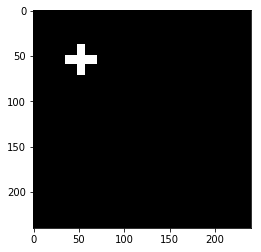
\includegraphics[width=\linewidth]{chapters/06_hdm/testnet/4.png}
        \caption{Ground truth segment}
    \end{subfigure}\hfill%
    \begin{subfigure}[t]{.34\textwidth}
        \centering
        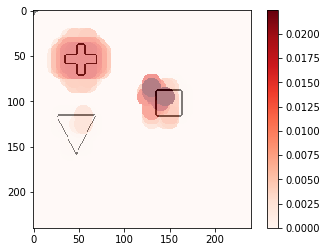
\includegraphics[width=\linewidth]{chapters/06_hdm/testnet/6.png}
        \caption{Regions where the applied masks reduce the accuracy of the segmentation}
    \end{subfigure}\hfill%
    \begin{subfigure}[t]{.34\textwidth}
        \centering
        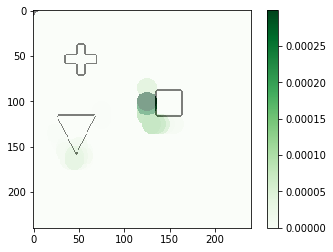
\includegraphics[width=\linewidth]{chapters/06_hdm/testnet/7.png}
        \caption{Regions where the applied masks increase the accuracy of the segmentation}
    \end{subfigure}
    \caption{Similar to above, both the visualizations (b) and (c) show that both the segmentation region itself and the square are important for the correct segmentation. In comparision to figure \ref}
\end{figure}

\begin{figure}[H]
    \centering
    \begin{subfigure}[t]{.28\textwidth}
        \centering
        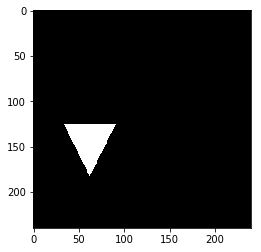
\includegraphics[width=\linewidth]{chapters/06_hdm/testnet/8.png}
        \caption{Ground truth segment}
    \end{subfigure}\hfill%
    \begin{subfigure}[t]{.34\textwidth}
        \centering
        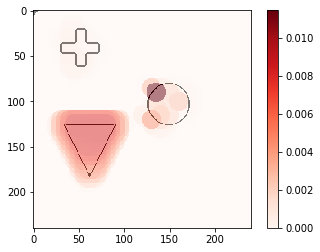
\includegraphics[width=\linewidth]{chapters/06_hdm/testnet/10.png}
        \caption{Regions where the applied masks reduce the accuracy of the segmentation}
    \end{subfigure}\hfill%
    \begin{subfigure}[t]{.34\textwidth}
        \centering
        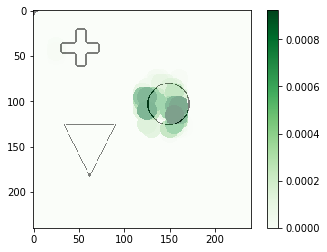
\includegraphics[width=\linewidth]{chapters/06_hdm/testnet/11.png}
        \caption{Regions where the applied masks increase the accuracy of the segmentation}
    \end{subfigure}
    \caption{TODO}
\end{figure}
